\documentclass[11pt,letterpaper]{article}
\usepackage[margin=0.86in]{geometry}
\usepackage[T1]{fontenc}
\usepackage[utf8]{inputenc}
\usepackage{lmodern}
\usepackage{xcolor}
\usepackage{tabularx,booktabs,array,longtable}
\usepackage{enumitem}
\usepackage{hyperref}
\usepackage{fancyhdr}
\usepackage{lastpage}
\usepackage{titlesec}
\usepackage{amsmath,amssymb}
\usepackage{microtype}
\usepackage{needspace}
\usepackage{ragged2e}
\usepackage{graphicx}
\definecolor{navy}{HTML}{19334C}
\definecolor{teal}{HTML}{236B82}
\definecolor{soft}{HTML}{EFF5F7}
\definecolor{muted}{HTML}{52616B}
\hypersetup{colorlinks=true,linkcolor=teal,urlcolor=teal}
\titleformat{\section}{\Large\bfseries\color{navy}}{\thesection.}{0.6em}{}
\titleformat{\subsection}{\large\bfseries\color{navy}}{\thesubsection}{0.6em}{}
\titleformat{\subsubsection}{\normalsize\bfseries\color{navy}}{\thesubsubsection}{0.6em}{}
\titlespacing*{\section}{0pt}{15pt}{6pt}
\titlespacing*{\subsection}{0pt}{10pt}{4pt}
\setlength{\parindent}{0pt}
\setlength{\parskip}{4.5pt}
\setlength{\headheight}{15pt}
\renewcommand{\arraystretch}{1.16}
\setlist[itemize]{topsep=3pt,itemsep=2pt,leftmargin=1.4em}
\setlist[enumerate]{topsep=3pt,itemsep=2pt,leftmargin=1.5em}
\pagestyle{fancy}
\fancyhf{}
\fancyhead[L]{\small\color{muted} Applied Machine Learning \textbar{} Cornell Tech}
\fancyhead[R]{\small\color{muted} Human or AI?}
\fancyfoot[C]{\small\color{muted} Page \thepage\ of \pageref{LastPage}}
\renewcommand{\headrulewidth}{0.3pt}
\newcommand{\placeholder}[1]{\par\noindent\textcolor{teal}{\textit{[Your response: #1]}}\par\vspace{0.3em}}
\newcommand{\figplaceholder}[1]{\par\noindent\fcolorbox{teal}{soft}{\parbox[c][1.15in][c]{0.94\linewidth}{\centering\textcolor{muted}{Insert #1 here}}}\par}
\newcommand{\question}[2]{\needspace{4\baselineskip}\par\addvspace{0.45em}\noindent\textbf{#1}\quad #2\par\nobreak\vspace{0.1em}}
\newcommand{\smallnote}[1]{{\small\color{muted}#1}}
\newcolumntype{Y}{>{\RaggedRight\arraybackslash}X}
\newcommand{\commit}[1]{\href{https://github.com/ZhenmanShen/human-or-ai-submissions/commit/#1}{\texttt{\detokenize{#1}}}}
\begin{document}
\thispagestyle{empty}
\vspace*{0.2in}
{\color{teal}\bfseries CORNELL TECH \textbar{} APPLIED MACHINE LEARNING}\par
\vspace{0.15in}
{\Huge\bfseries\color{navy} Human or AI?}\par
\vspace{0.07in}
{\LARGE\color{navy} Kaggle Competition Report --- Pretrained-model track}\par
\vspace{0.17in}

\textbf{Report Template: }\href{https://www.overleaf.com/project/6ae1fc85355dcf680137d898/share#f2777b20d3adeeecfac9096f78008e2f8daa0ff4be43de3b}{TEMPLATE}

\textbf{Github Repository Template: }\href{https://github.com/sekhari/human-or-ai-submissions}{REPO}

This track detects AI-written passages with features from frozen pretrained language models (GPT-2 token statistics, Qwen2.5 Binoculars scores) and with fine-tuned encoders (RoBERTa, DeBERTa-v3, the OpenAI GPT-2-output detector), combined in a rank/CDF blend. Because every reasonable model is near-perfect on held-out training data, the final blend was chosen on a held-out out-of-distribution proxy instead. All numbers below are re-measured on the team's fixed 2,000-row validation split, which the classical (from-scratch) track shares.

\vspace{0.06in}
\begin{tabularx}{\linewidth}{@{}>{\bfseries}p{1.58in}Y@{}}
Team / members & [TODO: names and NetIDs] \\
Kaggle team name & [TODO: Kaggle team name] \\
GitHub PR URL & [TODO: PR URL] \\
\end{tabularx}
\vspace{0.06in}
\subsection*{Your data}
\begin{tabularx}{\linewidth}{@{}lrrY@{}}
\toprule
\textbf{File} & \textbf{Rows} & \textbf{Labels} & \textbf{Purpose} \\
\midrule
\texttt{train.csv} & 10,000 & Visible & Supervised model development: 5,000 human (0), 5,000 AI (1) \\
\texttt{unlabeled.csv} & 3,000 & Hidden & Optional input for semi-supervised methods; required experiment \\
\texttt{test.csv} & 3,000 & Hidden & Predict the probability of AI authorship for Kaggle \\
\texttt{train\_starter\_2000.csv} & 2,000 & Visible & Convenient subset of \texttt{train.csv} for quick experiments \\
\bottomrule
\end{tabularx}

\smallnote{The starter data is a subset, not 2,000 additional labeled examples. Passages are approximately 75--350 words, with mean length near 210 words.}

\subsection*{How the test set works}
The test set mixes familiar and unfamiliar writing domains and AI generators, and includes some adversarially modified AI-written passages. You will \emph{not} receive labels, source model names, domain labels, or difficulty memberships for individual test examples. Submit a probability in $[0,1]$ for each test ID, where 1 means AI-generated. Kaggle evaluates submissions using \textbf{area under the ROC curve (AUROC)}. The \textbf{public leaderboard} covers 900 examples (30\%); the \textbf{private leaderboard} covers 2,100 (70\%) and determines the final competition performance score.

\vfill
\newpage
\section{Competition rubric and submission instructions}
\smallnote{Rubric and instructions as in the official template (Kaggle 25, model comparison 15, data size 10, unlabeled data 5, generalization 20, open-ended 15, code/PR 10). Validation protocol used throughout: fixed stratified 2,000-row split of \texttt{train.csv}, seed 20261023 (\texttt{common/val\_ids.csv}).}

\section{Team information and model summary}
\question{Q0.1 [0 points].}{List team members and their main contributions.}
[TODO: names, NetIDs and contributions.] The pretrained-track pipeline, experiments and this draft were produced with Claude Code (see Q6.3).

\question{Q0.2 [0 points].}{Summarize your final approach in 3--5 sentences. What is the overall pipeline from raw text to probability?}
Each passage is scored by seven models: three gradient-boosted (LightGBM) heads on frozen-LM features (GPT-2-medium token log-probability/rank/entropy statistics; Binoculars scores from Qwen2.5-0.5B and -1.5B base/instruct pairs; each plus 43 stylometric features), one GPT-2 head on token statistics alone, and three fine-tuned encoders (RoBERTa-base, DeBERTa-v3-large, the OpenAI GPT-2-output detector, RoBERTa-large). Every model's score is mapped through the empirical CDF of its own out-of-fold training scores, and the final probability is the weighted mean of these percentiles with weights 3, 3, 2, 1, 1, 1, 1 (blend A). The weights were chosen by greedy forward selection on a held-out proxy built from AI text of seven unseen generators and held-out human poetry and fiction, because training-set cross-validation could not separate the candidates.

\question{Q0.3 [0 points].}{Record your final scores (enter private score only once it is revealed).}
\begin{tabularx}{\linewidth}{@{}Yp{1.8in}@{}}\toprule Metric & Your score \\ \midrule Validation AUROC (blend A, fixed 2,000 rows) & 0.99990 \\ Kaggle public AUROC & 0.99161 \\ Kaggle private AUROC & [TODO: after reveal] \\ \bottomrule\end{tabularx}

\newpage
\section{Model comparison and selection (15 points)}
\textbf{Learning goal:} demonstrate sensible representation choices, comparisons of at least three approaches, appropriate hyperparameter selection, and evidence-based selection of the final classifier.

\question{Q1.1 [3 points].}{How did you preprocess and represent the text? Specify tokenization, normalization, word/character features or embeddings, and any feature extraction choices. Why?}
Text is used as given (only leading/trailing whitespace stripped): exploratory analysis showed formatting carries class signal (blank lines in about 66\% of AI and almost no human training passages), and Q5 confirms removing it hurts. Three representations are combined. (1) LM statistics: each passage is tokenised with the LM's own tokenizer (max 512 tokens) and summarised by mean/std/quantiles of token log-probability, rank and entropy; Binoculars adds the cross-perplexity ratio of a base/instruct Qwen2.5 pair. These measure how predictable the text is to an LM, which transfers across topics. (2) 43 stylometric features (length, sentence-length burstiness, type--token ratio, repetition, punctuation, blank lines) appended to (1); a 92-feature extended set (adding function words and readability) is the \texttt{stylometric\_gbm\_ext} baseline. (3) Fine-tuned encoders read sub-word tokens (512) end to end. A TF-IDF word 1--2/char 3--5 baseline is included for reference.

\question{Q1.2 [5 points].}{Which \textbf{three or more} modeling approaches did you try? Keep the labeled validation partition fixed across models.}
\begin{tabularx}{\linewidth}{@{}p{1.36in}Yrrr@{}}\toprule
Model & Text representation & Train AUROC & Val. AUROC & Train time \\ \midrule
\texttt{tfidf\_logreg} & word 1--2 + char\_wb 3--5 TF-IDF $\to$ LR & 1.00000 & 0.96093 & 21 s \\
\texttt{stylometric\_gbm\_ext} & 92 stylometric features $\to$ LightGBM & 1.00000 & 0.99836 & 7 s \\
\texttt{lm\_gpt2} & GPT-2 token log-prob/rank/entropy stats + style $\to$ LightGBM & 1.00000 & 0.99972 & 4 s \\
\texttt{lm\_gpt2\_nostyle} & GPT-2 token stats only $\to$ LightGBM & 0.99880 & 0.98591 & 1 s \\
\texttt{lm\_gpt2\_medium} & GPT-2-medium token stats + style $\to$ LightGBM & 1.00000 & 0.99970 & 4 s \\
\texttt{binoculars\_qwen05b} & Qwen2.5-0.5B Binoculars + token stats + style $\to$ LightGBM & 1.00000 & 0.99978 & 4 s \\
\texttt{binoculars\_qwen15b} & Qwen2.5-1.5B Binoculars + token stats + style $\to$ LightGBM & 1.00000 & 0.99970 & 4 s \\
\texttt{ft\_roberta\_base} & fine-tuned RoBERTa-base (512 tokens) & 0.99997 & 0.99812 & 4.1 min \\
\texttt{ft\_deberta\_v3\_large} & fine-tuned DeBERTa-v3-large (512 tokens) & 0.99877 & 0.99613 & 40.1 min \\
\texttt{ft\_openai\_detector\_large} & fine-tuned OpenAI GPT-2-output detector (RoBERTa-large) & 0.99935 & 0.99836 & 9.2 min \\
\midrule
Blend A (final) & blend A: 7 models, proxy-greedy weights (3,3,2,1,1,1,1) & 1.00000 & 0.99990 & 53.6 min \\
Blend B & blend B: 4 LM-feature models, equal weights & 1.00000 & 0.99985 & 16 s \\
Blend C & blend C: B + RoBERTa-base, equal weights & 1.00000 & 0.99987 & 4.3 min \\

\bottomrule\end{tabularx}
\smallnote{Train = the fixed 8,000 rows, Val = the fixed 2,000 rows, seed 20261023. Train time is the fit on the 8,000 rows; LM-feature models read cached LM features, so their time is the LightGBM head only (one full 5-fold run including feature extraction took 1.3--30 min, \texttt{cv5\_run\_time\_s\_seed42} in \texttt{results/fixed\_split/models.csv}). Blends apply the uploaded weights to the members' validation scores (weighted mean of percentile ranks); their time is the sum of the members'. GPUs: RTX 5070 (DeBERTa-v3-large on an RTX 3060).}

\textbf{The six submitted models, both tracks, same validation rows} (\texttt{common/compare\_tracks.py}):

{\small\begin{tabularx}{\linewidth}{@{}Ylrrrlr@{}}\toprule
Model & Track & Train & Val. & Train time & Hardware & Kaggle public \\ \midrule
Blend A & pretrained & 1.00000 & 0.99990 & 53.6 min & RTX 5070 + RTX 3060 & 0.99161 \\
Blend B & pretrained & 1.00000 & 0.99985 & 16 s & RTX 5070 + RTX 3060 & 0.98848 \\
Blend C & pretrained & 1.00000 & 0.99987 & 4.3 min & RTX 5070 + RTX 3060 & 0.98845 \\
C1 TF-IDF + LR & classical & 1.00000 & 0.96256 & 16 s & CPU & pending upload \\
C2 stylometric GBM & classical & 1.00000 & 0.99831 & 7 s & CPU & pending upload \\
C3 Transformer (scratch) & classical & 0.99787 & 0.98500 & 38 s & RTX 5070 & pending upload \\

\bottomrule\end{tabularx}}

\begin{center}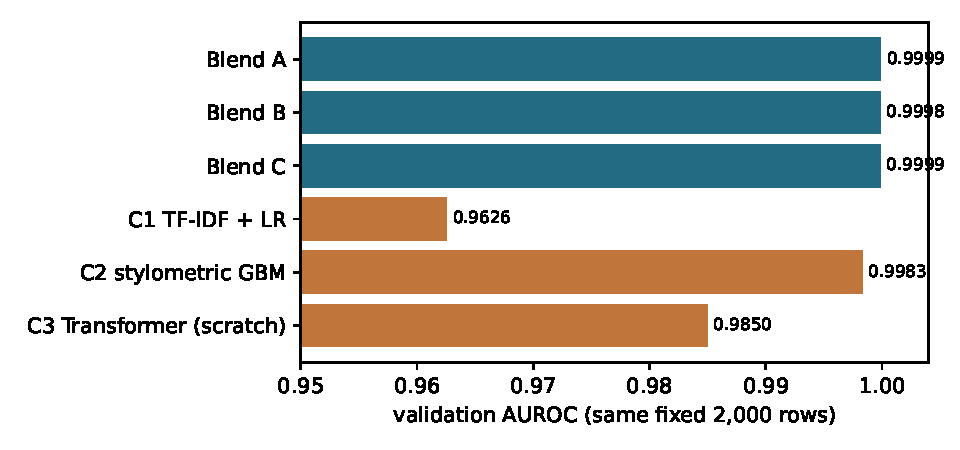
\includegraphics[width=0.49\linewidth]{../../common/figures/six_models.pdf}\hfill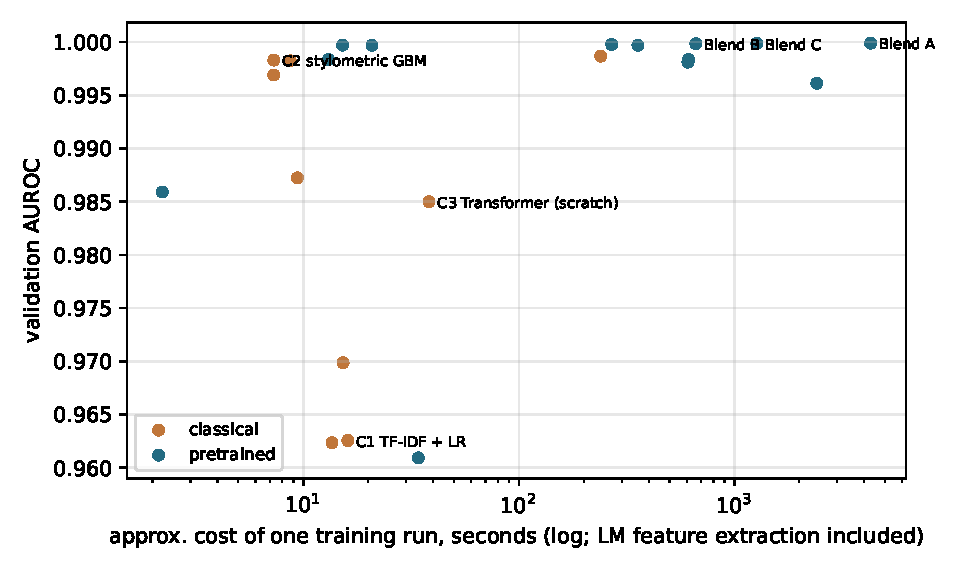
\includegraphics[width=0.49\linewidth]{../../common/figures/cost_vs_auroc.pdf}\end{center}

\textbf{Fixed split vs.\ the research repo's 5-fold CV.} The models were first developed with 5-fold stratified CV on all 10,000 rows (seed 42). Re-measured on the fixed split, the numbers agree to within 0.001 except TF-IDF (+0.003) and the OpenAI detector (+0.006); we report the fixed-split numbers.

{\small\begin{tabularx}{\linewidth}{@{}Yrrr@{}}\toprule Model & 5-fold CV (seed 42) & Fixed-split val & Difference \\ \midrule
\texttt{tfidf\_logreg} & 0.95764 & 0.96093 & +0.0033 \\
\texttt{stylometric\_gbm\_ext} & 0.99836 & 0.99836 & +0.0000 \\
\texttt{lm\_gpt2} & 0.99935 & 0.99972 & +0.0004 \\
\texttt{lm\_gpt2\_nostyle} & 0.98480 & 0.98591 & +0.0011 \\
\texttt{lm\_gpt2\_medium} & 0.99924 & 0.99970 & +0.0005 \\
\texttt{binoculars\_qwen05b} & 0.99924 & 0.99978 & +0.0005 \\
\texttt{binoculars\_qwen15b} & 0.99920 & 0.99970 & +0.0005 \\
\texttt{ft\_roberta\_base} & 0.99851 & 0.99812 & -0.0004 \\
\texttt{ft\_deberta\_v3\_large} & 0.99511 & 0.99613 & +0.0010 \\
\texttt{ft\_openai\_detector\_large} & 0.99276 & 0.99836 & +0.0056 \\

\bottomrule\end{tabularx}}

\question{Q1.3 [4 points].}{For at least \textbf{two} approaches, which hyperparameters and candidate values did you try? How did you select the final settings without using Kaggle test labels?}
\begin{tabularx}{\linewidth}{@{}p{1.18in}Yp{1.6in}@{}}\toprule Model & Parameters/values searched & Chosen setting \\ \midrule
\texttt{tfidf\_logreg} & C $\in$ \{0.5, 2, 4, 16, 64\} $\times$ word n-grams \{(1,1), (1,2)\}; 10 settings & C = 64, word [1,2]; inner CV 0.9562 \\
\texttt{lm\_gpt2} & num\_leaves \{7, 15, 31, 63\} $\times$ learning\_rate \{0.03, 0.1\} $\times$ n\_estimators \{200, 500, 1000\}; 24 settings & 63 leaves, lr 0.03, 500 trees; inner CV 0.9992 \\

\bottomrule\end{tabularx}

Each setting was scored by 5-fold stratified cross-validation inside the 8,000 training rows only (a dedicated \texttt{cv.scheme=inner} that puts the 2,000 validation rows in no fold, so they are never trained on or scored); the best mean fold AUROC wins. The validation set was used once afterwards, to report the chosen setting (TF-IDF 0.9611, \texttt{lm\_gpt2} head 0.9998), never to choose. For TF-IDF, bigrams beat unigrams at every C and C = 64 sits at the edge of the grid. The LM head is insensitive: all 24 settings lie between 0.9990 and 0.9992, so the remaining error is not in the head. Fine-tunes kept fixed epochs (no early stopping on validation).

\question{Q1.4 [3 points].}{Which approach did you choose for your final submission? Explain using validation performance, computational cost and/or stability. If you later changed the model, explain why.}
The final submission is blend A. In-distribution validation cannot justify that choice: blends A, B and C score 0.99990, 0.99985 and 0.99987 on the fixed split, and the best single model (Binoculars-Qwen-0.5B) 0.99978, differences far below what 2,000 rows can resolve. We therefore selected on the held-out OOD proxy (Q5), where A scores 0.9928 vs 0.9906 (B) and 0.9910 (C); the Kaggle public leaderboard agreed (0.99161 vs 0.98848 and 0.98845). A is also the most expensive (about 54 GPU-minutes of fine-tuning on the 8,000 rows plus LM feature extraction), while B needs only frozen-LM features; B is the fallback if cost matters, at $-0.003$ public AUROC. We did not change the model after uploading. Full submission history: Appendix A.

\section{Effect of training data size (10 points)}
\textbf{Learning goal:} understand the effect of the number of labeled examples on fitting and generalization. This is an empirical exercise; no formal sample-complexity theory is required.

\question{Q2.1 [4 points].}{Choose one model configuration. Train it with 500, 1,000, 2,000, 5,000 and 8,000 examples sampled from your 8,000-row training partition. Keep the same validation set and hyperparameters.}
Configuration: \texttt{lm\_gpt2} (GPT-2 token statistics + stylometric features $\to$ LightGBM, default head). Subsets are nested and stratified (seed 20261023); TF-IDF LR is shown as a contrast.
\begin{tabularx}{\linewidth}{@{}rrrY@{}}\toprule Training rows & Training AUROC & Validation AUROC & Notes (optional) \\ \midrule
500 & 1.0000 & 0.9972 & TF-IDF LR val 0.8994 \\
1,000 & 1.0000 & 0.9986 & TF-IDF LR val 0.9242 \\
2,000 & 1.0000 & 0.9988 & TF-IDF LR val 0.9378 \\
5,000 & 1.0000 & 0.9995 & TF-IDF LR val 0.9511 \\
8,000 & 1.0000 & 0.9997 & TF-IDF LR val 0.9609 \\

\bottomrule\end{tabularx}
\question{Q2.2 [3 points].}{Insert a plot of training and validation AUROC versus training-set size.}
\begin{center}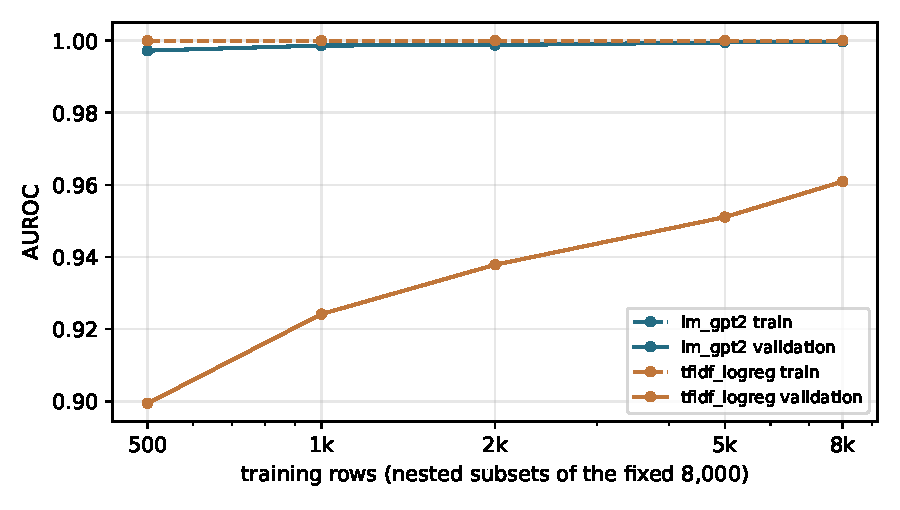
\includegraphics[width=0.72\linewidth]{figures/learning_curve.pdf}\end{center}
\question{Q2.3 [3 points].}{What does the curve suggest about overfitting, underfitting, and the value of more labeled examples?}
Training AUROC is 1.000 at every size for both models, so neither underfits: the trees and the high-dimensional linear model separate any training set this small perfectly, and the whole story is on the validation side. With LM features, 500 examples already reach 0.9972 and 8,000 reach 0.9997: the pretrained LM supplies the representation, and labels only calibrate a low-dimensional head, so the remaining gap is small and shrinking slowly (about +0.0002 from 5,000 to 8,000). TF-IDF is data-hungry (0.899 $\to$ 0.961) and still rising roughly linearly in $\log n$, the classic high-variance pattern. For the pretrained pipeline, more labels of the same kind are worth little; since test differs from train in domain and generator (Q5), more diverse data (new generators, verse) would plausibly help more than more of the same, but that is a hypothesis we did not test with training data.

\section{Learning from unlabeled data (5 points)}
\textbf{Learning goal:} test whether the additional 3,000 unlabeled passages help.
\question{Q3.1 [2 points].}{Describe one method that uses \texttt{unlabeled.csv} (e.g., self-training, confidence-based pseudo-labeling, clustering, or feature learning). How did you prevent validation-label leakage?}
Confidence-based pseudo-labelling: train on the 8,000 rows, score \texttt{unlabeled.csv}, add the 20\% highest-scored passages as AI and the 20\% lowest as human (1,200 in total), and refit; we ran 1 and 3 rounds (each round re-selects from the current model). Leakage control: the pool is \texttt{unlabeled.csv} only (no test or validation text); validation rows are excluded from training before anything is fit and are scored once at the end; and we checked that no unlabeled passage is identical to a validation passage (0 matches). Hyperparameters are those of the supervised baseline.
\question{Q3.2 [2 points].}{Compare against a supervised baseline under the same held-out validation protocol.}
\begin{tabularx}{\linewidth}{@{}Yp{1.5in}@{}}\toprule Method & Validation AUROC \\ \midrule
Supervised only (\texttt{lm\_gpt2}) & 0.9997 \\
Supervised only (\texttt{tfidf\_logreg}) & 0.9609 \\
Pseudo-labels, 1 round (\texttt{lm\_gpt2}) & 0.9997 \\
Pseudo-labels, 1 round (\texttt{tfidf\_logreg}) & 0.9603 \\
Pseudo-labels, 3 rounds (\texttt{lm\_gpt2}) & 0.9997 \\
Pseudo-labels, 3 rounds (\texttt{tfidf\_logreg}) & 0.9603 \\

\bottomrule\end{tabularx}
\question{Q3.3 [1 point].}{Did it help? Give a concrete, evidence-based explanation (including possible noise in pseudo-labels).}
No. \texttt{lm\_gpt2} moves by less than 0.00002 and TF-IDF loses 0.0006. The selected pseudo-labels are the passages the model is already sure about: for \texttt{lm\_gpt2} every selected unlabeled passage scored at least 0.9995 (AI) or at most 0.0005 (human), per the training log. Such examples carry almost no new information, and any that are wrong cannot be corrected by a model that put them there. \texttt{unlabeled.csv} also follows train's topic mix rather than test's (EDA), so it cannot teach the model the verse and fiction that test adds. Pseudo-label noise is not the issue here; uninformativeness is.

\newpage
\section{Generalization and error analysis (20 points)}
\textbf{Learning goal:} characterize how well the selected model generalizes and where it fails. Use \textbf{labeled validation data}; hidden test labels and hidden domain/generator information are unavailable.

\question{Q4.1 [5 points].}{Compare training and validation AUROC for your final selected model. Is there a gap? What explanations are plausible?}
Blend A has training AUROC 1.00000 (0.999997) and validation AUROC 0.99990, a gap of 0.0001; at a 0.5 threshold on its blended score it misclassifies 9 of 2,000 validation passages (3 FP, 6 FN). The in-distribution gap is negligible because the pretrained LMs provide features that do not depend on the training labels, and the LightGBM heads are fit to a well-sampled distribution. The relevant gap is to test: 0.99990 on validation vs 0.99161 on the public leaderboard. The plausible explanation, supported by the OOD proxy (Q5), is distribution shift: test contains unseen generators and much more creative writing and verse (16.6\% verse-like passages vs 1.6\% of training rows), on which every model is weaker. The validation split comes from the same distribution as training and cannot show this.

\question{Q4.2 [5 points].}{Evaluate performance over at least three text-length bins (define the bins), or another observable subgroup available in your data. Explain why you chose the grouping.}
\begin{tabularx}{\linewidth}{@{}Yrr@{}}\toprule Subgroup / bin & Count & Validation AUROC \\ \midrule
$<$150 words (word count; 234 AI) & 380 & 1.00000 \\
150-250 words (word count; 444 AI) & 1049 & 0.99986 \\
$>$250 words (word count; 322 AI) & 571 & 0.99999 \\
prose (line structure; 804 AI) & 1400 & 0.99983 \\
short lines (lists, recipes) (line structure; 192 AI) & 575 & 1.00000 \\
verse (line structure; 4 AI) & 25 & 1.00000 \\

\bottomrule\end{tabularx}
Length bins are $<$150, 150--250 and $>$250 words (LM statistics are averages, so short texts should be noisier). Line structure matters because by our heuristic ($\ge$4 lines, median $\le$10 words per line, no digits) test is 16.6\% verse (498 passages) against 1.6\% of the training rows, and validation has only 25 such passages, 4 of them AI (\texttt{common/results/split\_profile.csv}); short-line lists and recipes form a separate group. Blend A is at or above 0.9998 in every group, so no length or layout subgroup of the validation data exposes a weakness; the verse estimate rests on 25 rows and is not informative. This is itself the finding: the subgroup that matters most for test is almost absent from labelled data.

\question{Q4.3 [5 points].}{Analyze at least \textbf{five false positives and five false negatives} from your held-out validation set. Provide example IDs, predicted probabilities, and short failure hypotheses. Do not paste full passages unless essential.}
{\small\begin{tabularx}{\linewidth}{@{}p{0.5in}p{0.82in}p{0.42in}Y@{}}\toprule ID & Error type & P(AI) & Possible reason \\ \midrule
\mbox{2696} & FP & 0.583 & Run-on, repetitive predictive-text-style ramble with no punctuation; DeBERTa and the GPT-2 token-stats-only model rank it 0.87-0.93 - repetitive low-perplexity text looks like small-model AI output. \\
\mbox{6479} & FP & 0.505 & Wire-style football news report with quotes (Solskjaer injury); every member sits near 0.5 - formulaic news prose is predictable to an LM. \\
\mbox{7384} & FP & 0.505 & Short, informal movie review with run-on sentences; members split around 0.5 - hypothesis: generic review phrasing is low-surprise for the LMs. \\
\mbox{9388} & FP (near miss) & 0.495 & Near miss (P=0.495, below 0.5): Wikipedia bio of composer Bright Sheng with a long list of orchestras; list-like encyclopedic prose is predictable. \\
\mbox{6138} & FP (near miss) & 0.489 & Near miss (P=0.489): Wikipedia article on a paramilitary group; formal encyclopedic register, like 9388. \\
\mbox{6331} & FN & 0.476 & AI bread recipe with ingredient lines and self-correcting notes ('it was my error to add...'); the token-stats-only model ranks it 0.17 - hypothesis: messy, human-like asides and recipe layout. \\
\mbox{2914} & FN & 0.487 & AI physics proposal with hard line wraps and two-space indentation like an arXiv abstract; DeBERTa ranks it 0.05 - hypothesis: copies human arXiv formatting and dense jargon (high perplexity). \\
\mbox{3938} & FN & 0.494 & AI wiki-style article (View Askew universe) with long lists of film titles; all members near 0.5 - proper-noun lists look human to token statistics. \\
\mbox{7049} & FN & 0.494 & AI spelt-dough recipe with bullet glyphs and scraped-web layout (also a stylo\_gbm FN); formatting mimics human scraped text. \\
\mbox{1602} & FN & 0.496 & AI wiki-bio with a hatnote and [1] citation markers (also a stylo\_gbm FN); copies Wikipedia scraping artefacts that train associates with human text. \\

\bottomrule\end{tabularx}}
\smallnote{Threshold 0.5 on blend A's score (weighted mean of member percentiles). Blend A makes only 3 false positives at 0.5, so the two highest-scored human passages below the threshold are added as near misses. Member ranks per error: \texttt{results/error\_analysis/fp\_fn.csv}.}

\question{Q4.4 [5 points].}{What recurring failure patterns did you identify, and how might you address one of them? Distinguish observed patterns from speculation.}
\textit{Observed.} (1) Every error sits between 0.48 and 0.58: the blend's mistakes are disagreements between members, not confident errors; on 2696 and 2914 DeBERTa ranks the passage at 0.87 and 0.05 while the Binoculars and GPT-2-medium members sit at 0.52--0.56. (2) Four of five false negatives are AI passages formatted like scraped web text (recipe ingredient lines, a Wikipedia hatnote with \texttt{[1]} citations, arXiv-style hard line wraps, bullet glyphs); two of them (1602, 7049) are also among the classical stylometric model's top errors. (3) The false positives are formal, predictable human prose (news, encyclopedia, a generic review) and one repetitive ramble. \textit{Speculation.} The formatting copies human training artefacts that the models learned as human cues, and predictable human prose has the low perplexity LM features associate with AI. \textit{One fix to test:} augment AI training passages with scraped-web formatting (inserted citation markers, hard wraps, bullets) so the formatting cue stops implying ``human'', and measure the effect on the proxy and on these rows.

\newpage
\section{Open-ended improvements and insights (15 points)}
\textbf{Learning goal:} propose and test one improvement beyond the required baseline comparisons. This can be simple: a targeted feature change, alternate regularization scheme, ensemble, different representation, augmentation, or training approach. Sophistication alone does not earn credit.

\question{Q5.1 [3 points].}{What specific question or hypothesis motivated your improvement? What weakness or opportunity did you observe?}
After the full benchmark every reasonable model scored at least 0.990 in cross-validation and the best dozen runs lay within 0.0005 of each other (0.9988--0.9993, fold standard deviation about 0.0005), so CV could not rank them. Yet test differs from train: unseen generators, about 41\% creative writing versus 6.5\% (topic clusters, research-repo EDA), and 16.6\% verse-like passages versus 1.6\% (\texttt{common/results/split\_profile.csv}). Hypothesis: a held-out set that imitates this shift ranks models and blends differently from CV, and choosing the blend on it improves the leaderboard score, which CV-based selection cannot do.

\question{Q5.2 [4 points].}{What exactly did you change? Describe the baseline, the new approach and what you held fixed for a fair comparison.}
We built an evaluation-only proxy (\texttt{scripts/build\_eval\_set.py}, \texttt{eval\_ood.py}): 542 rewrites of training human passages and 816 poems and stories from seven local generators never used for training (Llama-3.2-3B, Qwen3-4B, Phi-3.5-mini, SmolLM2-1.7B, Granite-3.1-2B, OLMo-2-1B, Pythia-1.4B), plus 681 human poems and stories from held-out Project Gutenberg books. \texttt{proxy\_auc} pools these with out-of-fold training scores, weighted like test (41\% creative). Every candidate was scored by fold models that never saw the passage's source. Baseline: blend B, the equal-weight blend of the four best LM-feature models, chosen without the proxy. New approach: blend A, greedy forward selection on \texttt{proxy\_auc} over the 18 OOD-evaluated models and their variants. Held fixed: the trained models, the CDF blending rule and the training data. External text was used for evaluation only.

\question{Q5.3 [4 points].}{What were the measured results?}
{\small\begin{tabularx}{\linewidth}{@{}YrrY@{}}\toprule Configuration & Val. AUROC & Runtime & Relevant difference \\ \midrule
Baseline: blend B (equal weights, no eval-set tuning) & 0.99985 & 16 s & proxy 0.9906; unseen-generator 0.9958; Kaggle public 0.98848 \\
Improvement: blend A (greedy weights on the OOD proxy) & 0.99990 & 53.6 min & proxy 0.9928; unseen-generator 0.9970; Kaggle public 0.99161 \\

\bottomrule\end{tabularx}}
\smallnote{Val.\ = fixed 2,000 rows; runtime = summed fit time on the 8,000 rows. Proxy and unseen-generator AUROC from \texttt{experiments/ood\_eval.csv}.}

Two negative results from the same programme. Removing formatting cues (``debiased'': blank lines, double spaces, quotes, zero-width characters, homoglyphs) or joining all lines (removing the verse-like line structure):
{\small\begin{tabularx}{\linewidth}{@{}Yrr@{}}\toprule Model, variant & Fixed-split val AUROC & OOD proxy AUROC \\ \midrule
\texttt{stylometric\_gbm\_ext}, as is & 0.9984 & 0.9741 \\
\texttt{stylometric\_gbm\_ext}, debiased & 0.9963 & 0.9148 \\
\texttt{stylometric\_gbm\_ext}, join\_lines & 0.9790 & -- \\
\texttt{lm\_gpt2}, as is & 0.9997 & 0.9887 \\
\texttt{lm\_gpt2}, debiased & 0.9988 & 0.9683 \\
\texttt{lm\_gpt2}, join\_lines & 0.9949 & -- \\

\bottomrule\end{tabularx}}

\question{Q5.4 [4 points].}{What did you learn? Did the results support the hypothesis? What limits the conclusion, and what would you try next?}
The hypothesis held as far as we can test it. The proxy ranked the candidates differently from CV: the old CV-greedy blend was the best on CV (0.99964) but scored 0.9862 on the proxy. It also put A first, and Kaggle agreed (public 0.99161 vs 0.98848). The fixed split could not see any of this: A and B differ by 0.00005 on validation. The proxy was 0.001--0.003 above the public scores, while CV was 0.008--0.011 above. Limits: the selection is in-sample for the proxy, so A's proxy score is optimistic; the proxy's generators and its archaic Gutenberg humans are our guess at test, not test; and one public-leaderboard comparison on 900 rows is weak evidence, which the private score will test. The debiasing results are negative and informative: formatting cues still help on unseen generators (stylometric proxy 0.974 $\to$ 0.915 when removed), so they are signal, not just a training-set artefact. Next: the formatting augmentation from Q4.4, and selecting on half of the generators and scoring on the other half to measure the selection optimism.

\section{Code submission, reproducibility and AI assistance (10 points)}
\textbf{Submission format:} Submit a \textbf{GitHub PR URL} against the course repository. We will inspect the final code and its development history, not just the final snapshot. Do not squash away meaningful intermediate commits before review. Template \href{https://github.com/sekhari/human-or-ai-submissions}{here}.

\question{Q6.1 [5 points].}{Provide the PR URL, the entrypoint for training/evaluation, and the command used to generate \texttt{submission.csv}. State dependencies and random seeds.}
PR: [TODO: PR URL]. Code: \texttt{submissions/<team>/pretrained/} (Python 3.12, \texttt{pip install -r requirements.txt}; PyTorch with CUDA 12.8+ for an RTX 50-series GPU; Kaggle CSVs outside git via \texttt{--data-dir} or \texttt{HOA\_DATA\_DIR}).
\begin{itemize}
\item Fixed-split evaluation (all report tables): \texttt{python run\_all.py --profile fixed}, then \texttt{python scripts/report\_experiments.py collect --session outputs/sessions/<session>} and \texttt{hpsearch}, \texttt{curve}, \texttt{semisup}, \texttt{errors}, \texttt{debias}; \texttt{python scripts/report\_tables.py}.
\item Kaggle file: \texttt{python run\_all.py --profile ood} (5-fold models, about 4 h on two 12 GB GPUs), then \texttt{python make\_submission.py --run <7 runs> --weights 3 3 2 1 1 1 1 --name final\_A\_greedy\_proxy}, which writes \texttt{outputs/submissions/final\_A\_greedy\_proxy.csv} and validates it. The uploaded files are committed in \texttt{kaggle\_submissions/}.
\end{itemize}
Seeds: 20261023 for the split and every fixed-split experiment; the original 5-fold runs behind the uploaded files used seed 42 (fold $k$ seeded $42+k$). Fine-tunes use bf16 on GPU, so reruns differ in the last digits.

\question{Q6.2 [3 points].}{Give two or three examples of changes you made during development. Link to relevant commits or PR discussion and briefly explain what the experiments taught you.}
\begin{itemize}
\item \commit{1fc181fef044ef79830a9a0db09f32bc305f38e0} (full PC benchmark, 35 jobs): every reasonable model reached 0.990--0.999 CV AUROC with fold noise of about 0.0005. Lesson: training-set CV is saturated and cannot choose a model, so we needed an out-of-distribution evaluation.
\item \commit{ed4ad2daeabbb6f05fc791791dff0edf34ced42e} and \commit{77663a46bfcbc667df49d3aeb81d00485319b2f8} (held-out generator/creative proxy, blends chosen on it): the proxy ranking differed from the CV ranking: fine-tunes and the stylometric GBM tie the LM-feature models on CV but drop to 0.971--0.975 on the proxy and flag 42--74\% of held-out human poems and stories. The proxy-chosen blend A then won on Kaggle.
\item \commit{3754f3b7f2d07855ff6e01a9ef753e7f575d4698} and \commit{5941e57fa758b3624c5587f21f0f835c4c76fdf3} (negative results, re-measured on the fixed split): removing formatting cues and pseudo-labelling unlabeled text both failed to help. The formatting cues are real signal, and confident pseudo-labels add no information.
\end{itemize}

\question{Q6.3 [2 points].}{How did you use AI tools (such as Claude, ChatGPT or Copilot) for code, debugging, analysis or writing? What did you verify or modify yourself?}
[TODO: team to edit.] Claude Code (Anthropic) wrote most of the pipeline code, ran the experiments on our machines and drafted this report from the generated results files; every number in the tables is produced by scripts in the repository (\texttt{scripts/report\_tables.py}), not typed by hand. [TODO: what the team verified or changed themselves.] Pretrained weights used (Hugging Face): \texttt{openai-community/gpt2}, \texttt{openai-community/gpt2-medium}, \texttt{Qwen/Qwen2.5-0.5B}, \texttt{Qwen/Qwen2.5-0.5B-Instruct}, \texttt{Qwen/Qwen2.5-1.5B}, \texttt{Qwen/Qwen2.5-1.5B-Instruct}, \texttt{FacebookAI/roberta-base}, \texttt{microsoft/deberta-v3-large}, \texttt{openai-community/roberta-large-openai-detector}. The OOD proxy used text generated locally by seven open models and Project Gutenberg books, for evaluation and blend selection only, never as training labels. No external LLM API labelled or scored test passages, and no hidden labels were retrieved.

\textbf{AI policy.} You may use AI assistants for coding, debugging, explanations, brainstorming, and editing. We expect each team to exercise its own judgment, run experiments, check outputs, and understand its submitted approach. Sending the entire assignment to an AI tool and submitting its unverified output without meaningful involvement does not satisfy the objectives of this project. We will use the PR history, reproducible experiments and report together as evidence of engagement. \emph{Commit counts and the presence of AI-generated code are not themselves grading criteria.} Do not fabricate results or retrieve hidden test labels.

\section*{Final submission checklist}
\begin{itemize}[label=$\square$]
\item Final probabilities submitted to Kaggle for every \texttt{test.csv} ID.
\item Completed report, with all required answers, tables, figures and sources, submitted as PDF.
\item GitHub PR linked on the report title page and in the course submission portal.
\item Code and dependencies recreate final predictions (within reasonable numerical tolerance).
\item Relevant experiments and seed/configuration details are recorded.
\item AI-use disclosure is complete; hidden labels were not retrieved externally.
\end{itemize}

\appendix
\section*{Appendix A. Submission and testing history}
Generated from \texttt{submission\_log.csv} (also \texttt{SUBMISSIONS.md}); every model validated on the fixed split, both tracks. ``not submitted'' = tested only.

{\footnotesize\begin{longtable}{@{}llp{1.7in}lrll@{}}\toprule
Date & Track & Model & Commit & Val AUROC & Kaggle public & Private \\ \midrule\endhead
2026-10-31 & pretrained & \texttt{final\_A\_greedy\_proxy} & \href{https://github.com/ZhenmanShen/human-or-ai-submissions/commit/c7c1e3e5c379f092b31d1ef745dbf2900d052f03}{\texttt{c7c1e3e}} & -- & 0.99161 & -- \\
2026-10-31 & pretrained & \texttt{final\_B\_lm4} & \href{https://github.com/ZhenmanShen/human-or-ai-submissions/commit/c7c1e3e5c379f092b31d1ef745dbf2900d052f03}{\texttt{c7c1e3e}} & -- & 0.98848 & -- \\
2026-10-31 & pretrained & \texttt{final\_C\_lm4\_roberta} & \href{https://github.com/ZhenmanShen/human-or-ai-submissions/commit/c7c1e3e5c379f092b31d1ef745dbf2900d052f03}{\texttt{c7c1e3e}} & -- & 0.98845 & -- \\

\bottomrule\end{longtable}}

\end{document}
